% \IUref{IUAdmPS}{Administrar Planta de Selección}
% \IUref{IUModPS}{Modificar Planta de Selección}
% \IUref{IUEliPS}{Eliminar Planta de Selección}

% Copie este bloque por cada caso de uso:
%-------------------------------------- COMIENZA descripción del caso de uso.

%\begin{UseCase}[archivo de imágen]{UCX}{Nombre del Caso de uso}{
	\begin{UseCase}{CU22}{Baja de un curso}{
		Resumen:Cuando el Gerente de Sucursal elimina el registro de un curso en el sistema, se ingresan los datos: numero de curso o nombre de curso, costo, horario, fecha de inicio,area, fecha de termino,nombre de instructor y su  horario en formato 24:00. Este Curso sera buscado en la base de datos el cual arrojara la coinidencia exacta una vez Validado los 8 campos (todos obligatorios), que posteriormente sera eliminado del sistema.
		\begin{figure}
  		\centering
   		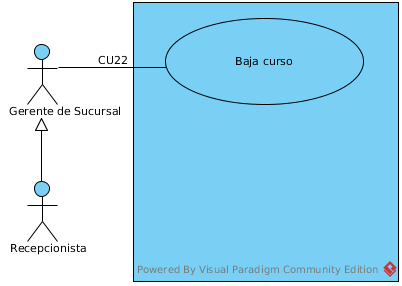
\includegraphics[width=0.4\textwidth]{images/CU22}
  		\caption{CU22 Baja de Curso}
		\end{figure}
	}
		\UCitem{Versión}{0.1}
		\UCitem{Actor}{Gerente de Sucursal}
		\UCitem{Propósito}{Eliminar de cursos en el sistema.}
		\UCitem{Entradas}{numero de curso(id), nombre de curso, costo, horario, fecha de inicio,area, fecha de termino,nombre de instructor y su  horario en formato 24:00}
		\UCitem{Origen}{Teclado}
		\UCitem{Salidas}{nombre de curso, costo, horario, fecha de inicio,area, fecha de termino,nombre de instructor y su  horario en formato 24:00 }
		\UCitem{Destino}{Pantalla}
		\UCitem{Precondiciones}{El curso debe de estar registrado en el sistema con los mismas descipciones.}
		\UCitem{Postcondiciones}{El Gerente de Sucursal dara de baja un registro de curso al sistema.}
		\UCitem{Errores}{Que no se tenga memoria disponible en el Disco.}
		\UCitem{Tipo}{Caso de uso primario}
		\UCitem{Observaciones}{Los cursos solo pueden ser eliminados por un Gerente de Sucursal.}
		\UCitem{Autor}{Carrillo Mendoza Martín Alejandro.}
		\UCitem{Reviso}{Carrillo Mendoza Martín Alejandro.}
	\end{UseCase}
	\newpage
	\begin{UCtrayectoria}{Principal}
	
	\UCpaso[\UCactor] Ingresa a la pagina web de \IUref{IU21.0}{Pantalla de Control de Acceso}\label{CU22.0Login} y proporciona su correspondiente nombre de usuario (username) y contraseña (password) para acceder al sistema.
		\UCpaso Válida que el actor se encuentre dado de alta en el sistema. Se utiliza la regla \BRref{BR117}{Determinar si el usuario tiene acceso al sistema.} \Trayref{A}.
		\UCpaso Despliega la \IUref{IU22.1}{Pantalla pestaña principal gerente de sucursal}, en ella se encuentran los campos: nombre de curso, costo, horario, fecha de inicio,area, fecha de termino,nombre de instructor y su  horario en formato 24:00, todos ellos obligatorios para la baja de un curso en el sistema.	
	\UCpaso[\UCactor] Al solicitar la baja de un curso a la base de datos,selecciona la pestaña " Baja de Curso  " de la IU21.1 de Menú principal.
	\UCpaso Despliega la \IUref{IU23.1}{Pantalla dar de baja Curso.}
	\UCpaso[\UCactor] Introduce los datos del curso a dar de baja, con su respectivo formato y tipo de dato solicitado, estos son: nombre de curso(varchar), costo(float), fecha de inicio(DATE), fecha de termino(DATE), costo(float).
    \UCpaso[\UCactor] Selecciona el nombre del instructor de curso.
	\UCpaso[\UCactor] Selecciona los dias ala semana en los que se imparte curso.
	\UCpaso[\UCactor] Selecciona la hora en que se imparte curso (los dias ya seleccionados previamente).
	\UCpaso[\UCactor] Selecciona el area donde se imparte el curso.
	\UCpaso[\UCactor] Confirma la baja de curso al sistema dando click al boton \IUbutton{Enviar} de \label{IU22.1 Baja Curso}.
	\UCpaso Verifica que todos los campos esten llenos ademas con el formato y tipo correspondiente a los datos ubucados en la base de datos. \BRref{BR118}{Validar los datos de un formulario} \Trayref{B}.
		
		\UCpaso Elimina el registro de curso en la base de datos.
		\UCpaso Muestra el \IUref{UI22.1}{Baja Exitosa de curso.}\Trayref{C}.
		\UCpaso Regresa a la pantalla principal de acceso a gerente de sucursal\IUref{IU21.1}{Pantalla de acceso a Gerente de Sucursal}.
\end{UCtrayectoria}

\begin{UCtrayectoriaA}{A}{El actor no introduce nombre de usuario (username) y contraseña (password) para poder ingresar al sistema.}
			\UCpaso Muestra el mensaje {\bf MSG22.0-}``Usuario [{\em y/o}] contraseñas no validos.''.
			\UCpaso[\UCactor] Oprimé el botón \IUbutton{Aceptar}.
			\UCpaso Regresa a la pantalla principal de acceso a gerente de sucursal\IUref{IU21.1}{Pantalla de acceso a Gerente de Sucursal}.
		\end{UCtrayectoriaA}

		\begin{UCtrayectoriaA}{B}{Almenos un campo no esta lleno o no tiene formato adecuado}
			\UCpaso Muestra el mensaje {\bf MSG22.1-}``Uno o más [{\em campos}] no tienen el formato adecuado''.ademas que se tiene obligatoriamente que llenar todos los campos.
			\UCpaso[\UCactor] Oprime el botón \IUbutton{Aceptar}
			\UCpaso[] Termina el caso de uso.
		\end{UCtrayectoriaA}
		
		\begin{UCtrayectoriaA}{C}{La baja del curso no fue realizada }
			\UCpaso Muestra el Mensaje {\bf MSG22.2-}El Curso [{\em nombre de curso, costo, horario, fecha de inicio,area, fecha de termino,nombre de instructor y su  horario en formato 24:00 }] no eliminado, compruebe el Disco.
			\UCpaso[\UCactor] Oprime el botón \IUbutton{Aceptar}
			\UCpaso[] Termina el caso de uso.
		\end{UCtrayectoriaA}	
%-------------------------------------- TERMINA descripción del caso de uso.